\documentclass[12pt, a4paper, brazil]{abntex2}
\usepackage[utf8]{inputenc}
\usepackage[T1]{fontenc}
\usepackage[left=2cm, top=3cm, right=2cm, bottom=2cm]{geometry}
\usepackage[normalem]{ulem}
\usepackage[dvipsnames]{xcolor}
\usepackage{graphicx}
\graphicspath{{./src/img/}}
\usepackage{float}

\usepackage[alf]{abntex2cite}

\usepackage{hyperref}
\hypersetup{
    colorlinks=true,
  linkcolor=black,
  citecolor=black,
  urlcolor=black
  }

\usepackage{indentfirst}
\usepackage{multicol}

\setlength{\columnseprule}{0.5pt}
\setlength{\columnsep}{25pt}

\usepackage{amsmath}
\usepackage{amsthm}
\usepackage{amsfonts}
\usepackage{amssymb}
\usepackage{xfrac}

\usepackage{enumitem}

\DeclareMathOperator{\sen}{sen}
\DeclareMathOperator{\tg}{tg}

\renewenvironment{proof}{\vspace{\onelineskip} \noindent{\bfseries Demonstração:}}{\qed}

\setcounter{tocdepth}{2}

\newcounter{questaovest}

\newcommand{\vest}[1]{\stepcounter{questaovest}\item[\textbf{Questão \arabic{questaovest}} (#1):]}
\setlist[enumerate]{
    align=left,
    leftmargin=*,
    }
    
\setlist[enumerate,2]{
    label=\alph*),
    font=\bfseries,
    itemsep=0.1pt,
    labelsep=0em,
    parsep=0pt,
    leftmargin=1.2em
    }
    
    
    \renewcommand{\bibsection}{%
  \chapter*[Referências]{Referências} % Na página e no cabeçalho
  \addcontentsline{toc}{chapter}{Referências} % No Sumário
  }

  \chapterstyle{companion}
  \renewcommand{\printchaptertitle}[1]{
  \begin{adjustwidth}{}{0pt}
    \raggedleft\chaptitlefont#1\par\nobreak
  \end{adjustwidth}
}

\hyphenation{Chla-my-dia}

\begin{document}
\begin{multicols*}{2}
    \begin{enumerate}
        \vest{UECE-2018} A soma de todas as frações da forma $\displaystyle \frac{n}{n+1}$, onde $n$ é um elemento do conjunto $\{1,2,3,4,5\}$, é:
        
        \begin{enumerate}
            \item 4,55
            \item 6,55
            \item 5,55
            \item 3,55
        \end{enumerate}

        \vest{ESPM-2016} Na multiplicação abaixo, cada letra representa um algarismo do sistema decimal de numeração. O valor de $A+B+C+D$ é:

        \[
        \begin{array}{r@{\quad}l}
            \text{A B C} & \\
            \times \quad 9 & \\
            \hline
            7\text{ D C }6
        \end{array}
        \]

        \begin{enumerate}
            \item 22
            \item 20
            \item 24
            \item 21
            \item 23
        \end{enumerate}


        \vest{ENEM-2017} A \textit{Chlamydia}, a menor bactéria do mundo, mede cerca de $0,2$ micrômetro ($1$ micrômetro equivale à milionésima parte de um metro). Para ter uma noçãode como é pequena a \textit{Chlamydia}, uma pessoa resolveu descrever o tamanho da bactéria na unidade milímetro.
        A medida da \textit{Chlamydia}, em milímetro, é:

        \begin{enumerate}
            \item $2 \times 10^{-1}$
            \item $2 \times 10^{-2}$
            \item $2 \times 10^{-4}$
            \item $2 \times 10^{-5}$
            \item $2 \times 10^{-7}$
        \end{enumerate}

        \columnbreak

        \vest{ENEM-2016} A London Eye é uma enorme roda-gigante na capital inglesa. Por ser um dos monumentos construídos para celebrar a entrada do terceiro milênio, ela também é conhecida como Roda do Milênio. Um turista brasileiro, em visita à Inglaterra, perguntou a um londrino o diâmetro (destacado na imagem) da Roda do Milênio e ele respondeu que tem $443$ pés.

            \begin{figure}[H]
                \centering
                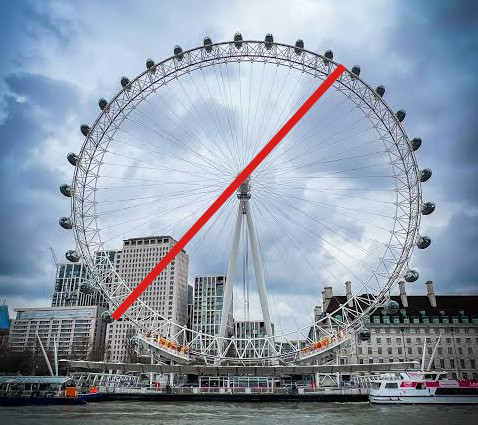
\includegraphics[width=0.4\textwidth]{london_eye.png}
                \caption{A Roda do Milênio}
                \label{fig:imagem01}
            \end{figure}
        

        Não habituado com a unidade pé, e querendo satisfazer sua curiosidade, esse turista consultou um manual de unidades de medidas e constatou que $1$ pé equivale a $12$ polegadas, e que $1$ polegada equivale a $2,54$ cm. Após alguns cálculos de conversão, o turista ficou surpreendido com o resultado obtido em metros.

        Qual a medida que mais se aproxima do diâmetro da Roda do Milênio, em metro?

        \begin{enumerate}
            \item $53$
            \item $94$
            \item $113$
            \item $135$
            \item $145$
        \end{enumerate}

        \newpage
        \vest{ENEM-2015} Um bairro residencial tem cinco mil moradores, dos quais mil são classificados como vegetarianos. Entre os vegetarianos, $40\%$ são esportistas, enquanto que, entre os não vegetarianos, essa porcentagem cai para $20\%$. Uma pessoa desse bairro, escolhida ao acaso, é esportista.
        A probabilidade de ela ser vegetariana é:

        \begin{enumerate}
            \item $ \displaystyle \frac{2}{25}$ \vspace{7pt}
            \item $\displaystyle \dfrac{1}{5}$ \vspace{7pt}
            \item $\displaystyle \dfrac{1}{4}$ \vspace{7pt}
            \item $\displaystyle \dfrac{1}{3}$ \vspace{7pt}
            \item $\displaystyle \dfrac{5}{6}$ \vspace{7pt}
        \end{enumerate}

        \vest{ENEM} Jogar baralho é uma atividade que estimula o raciocínio. Um jogo tracional de é a Paciência, que utiliza 52 cartas. Inicialmente são formadas sete colunas com as cartas. A primeira coluna tem uma carta, a segunda tem duas cartas, a terceira tem três cartas, a quarta tem quatro cartas, e assim sucessivamente até a sétima coluna, a qual tem sete cartas, e o que sobra forma o monte, que são as cartas não utilizadas nas colunas.
        A quantidade de cartas que forma o monte é:

        \begin{enumerate}
            \item $21$
            \item $24$
            \item $26$
            \item $28$
            \item $31$
        \end{enumerate}

        \columnbreak

        \vest{ENEM} Em canteiros de obras de construção civil é comum perceber trabalhadores realizando medidas de comprimento e de ângulos e fazendo demarcações por onde a obra deve começar ou se erguer. Em um desses canteiros foram feitas algumas marcas no chão plano. Foi possível perceber que, das seis estacas colocadas, três eram vértices de um triângulo retângulo e as outras três eram os pontos médios dos lados desse triângulo, conforme pode ser visto na figura, em que as estacas foram indicadas por letras.

            \begin{figure}[H]
                \centering
                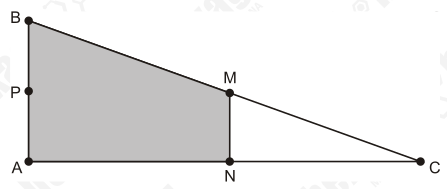
\includegraphics[width=0.4\textwidth]{triangulo.png}
            \end{figure}
        

        A região demarcada pelas estacas $A, B, M$ e $N$ deveria ser calçada com concreto.
        Nessas condições, a área a ser calçada corresponde:

        \begin{enumerate}
            \item a mesma área do triângulo $AMC$.
            \item a mesma área do triângulo $BNC$.
            \item a metade da área formada pelo triângulo $ABC$.
            \item ao dobro da área do triângulo $MNC$.
            \item ao triplo da área do triângulo $MNC$.
        \end{enumerate}

    \end{enumerate}
  \end{multicols*}
\end{document}